\documentclass[12pt,a4paper]{report}

\setlength{\parindent}{0pt} % get to fuck the paragraph indent

\usepackage[OT1]{fontenc}		% Font

\usepackage{verbatim}
\usepackage[utf8]{inputenc}

\usepackage[none]{hyphenat}
\usepackage{graphicx}				% Allows for photos to be added
%\usepackage{parskip} 				% Stops the horrific spacing 
\usepackage[top=0cm, foot=1.5em, bottom=2.5cm, left=2cm, right=2cm]{geometry} 	% Set margins to .5 inches 
\addtolength{\topmargin}{0.5in}		% Set top margin to 1 inch
\usepackage{hyperref}				% Hyperlinks package
\hypersetup{colorlinks=true, linkcolor=blue, citecolor = blue, filecolor=black, urlcolor=blue} 	% Make types of hyperlinks
\urlstyle{same}

\renewcommand*\familydefault{\sfdefault} 


\begin{document}


\begin{center}
\large \textbf{A System to Help Prevent Crashes in Rowing Boats \\ How to Construct Your Own System}
\end{center}
 
This is a 'how to' guide to building the nodes and downloading the software needed to build your very own MANET. Each node \emph{should} beep (or flash an LED, depending on what you choose) when the user is approaching a known obstacle, much like parking sensors on a car! A disclaimer - I do not guarantee this will work and take no responsibility for any collisions. \\ \\


\textbf{Components Needed} \\
This is a list of what I used in my project, and therefore what the software I wrote has been designed for. Any microcontroller, GPS and radio can be substituted.\begin{itemize} 
\item Raspberry Pi Pico
\item Adafruit RFM69HCW Transceiver Radio Breakout
\item Adafruit Ultimate GPS Breakout
\item Non-latching Button (mine has an LED ring around it used to tell if the node is on)
\item Buzzer and resistor (resistor moderates the pitch of the buzzer, I use 10k) 
\item Waterproof box
\item Power pack (to power the device)
\item 3M Dual Lock or other method of attaching the final node to the boat
\item Breadboard (optional but recommended)
\item Wires 
\end{itemize}
\bigskip


\textbf{Tools Needed} \\
\begin{itemize}
\item Soldering iron
\item Drill and bit of the same diameter as your button (I use 12mm)
\end{itemize}
\bigskip

\textbf{Wiring}
\begin{center}
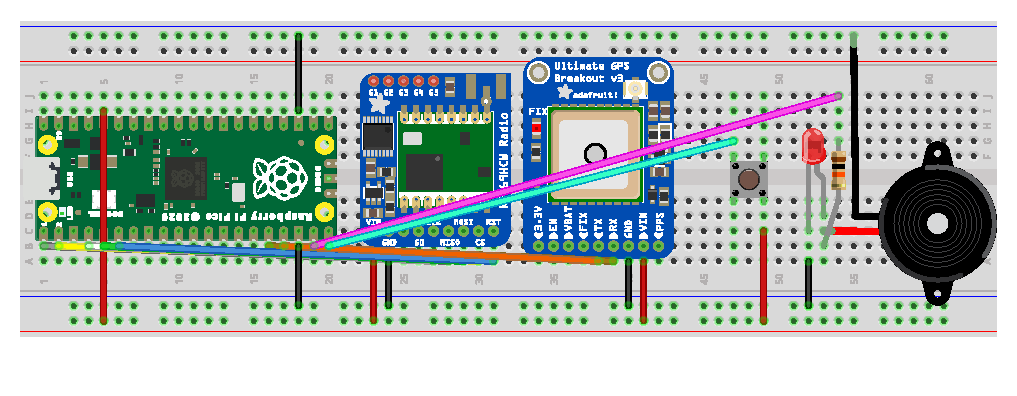
\includegraphics[scale = 0.5]{breadboard.pdf} \\
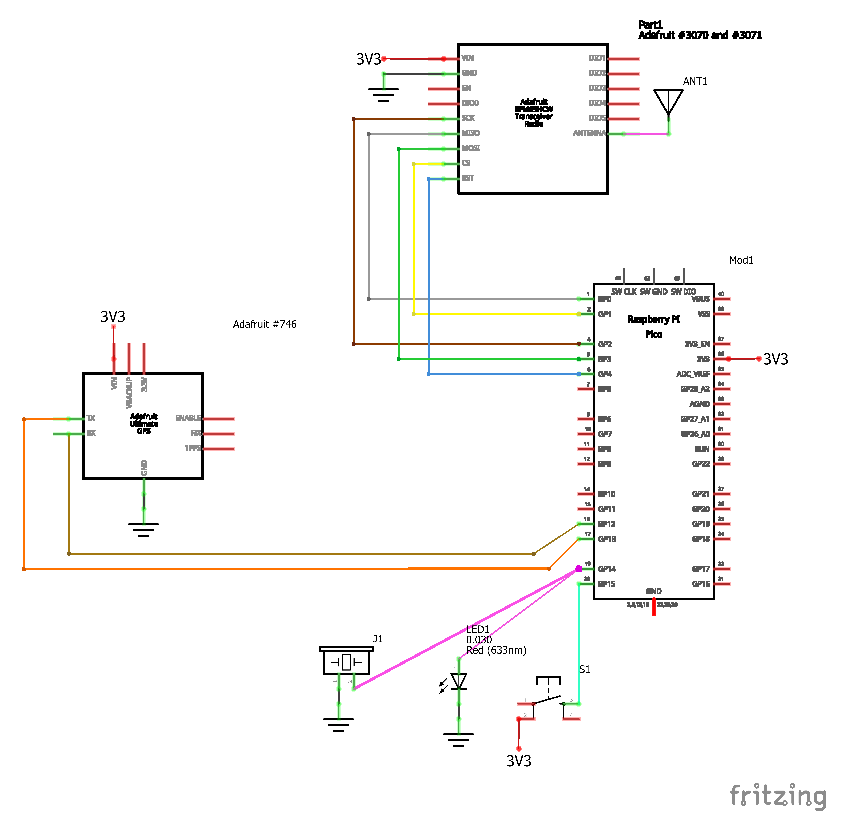
\includegraphics[scale = 0.5]{wiring.pdf}
\end{center}

\textbf{Software} \\
After running CircuitPython on your device (AdaFruit has a good little tutorial here: \url{https://learn.adafruit.com/getting-started-with-raspberry-pi-pico-circuitpython/circuitpython}) 
Go to the OnDevice folder in this repository and upload the boot.py file and deviceCode.py to the Pico, then place the contents of the lib folder into the Pico's lib folder. When you're done, the Pico's filesystem should read:

\begin{verbatim}
boot.py
deviceCode.py

lib
    adafruit_gps.py
    rfm69.py
    config.py
\end{verbatim}

You'll need to go into \verb`lib > config.py` and manually set the \verb`ADDRESS` constant to a unique value for each node. Remember each address must be smaller than 0xFE, 254!   \\

If you want to change any other parameters, they are all held in the config.py file, with comments above. Simply plug the device into your computer and edit. \\ \\

\textbf{SetUp} \\
As the button and any LEDs need to be on the outside of the box, you'll have to drill a hole into your waterproof box.  
\begin{center}
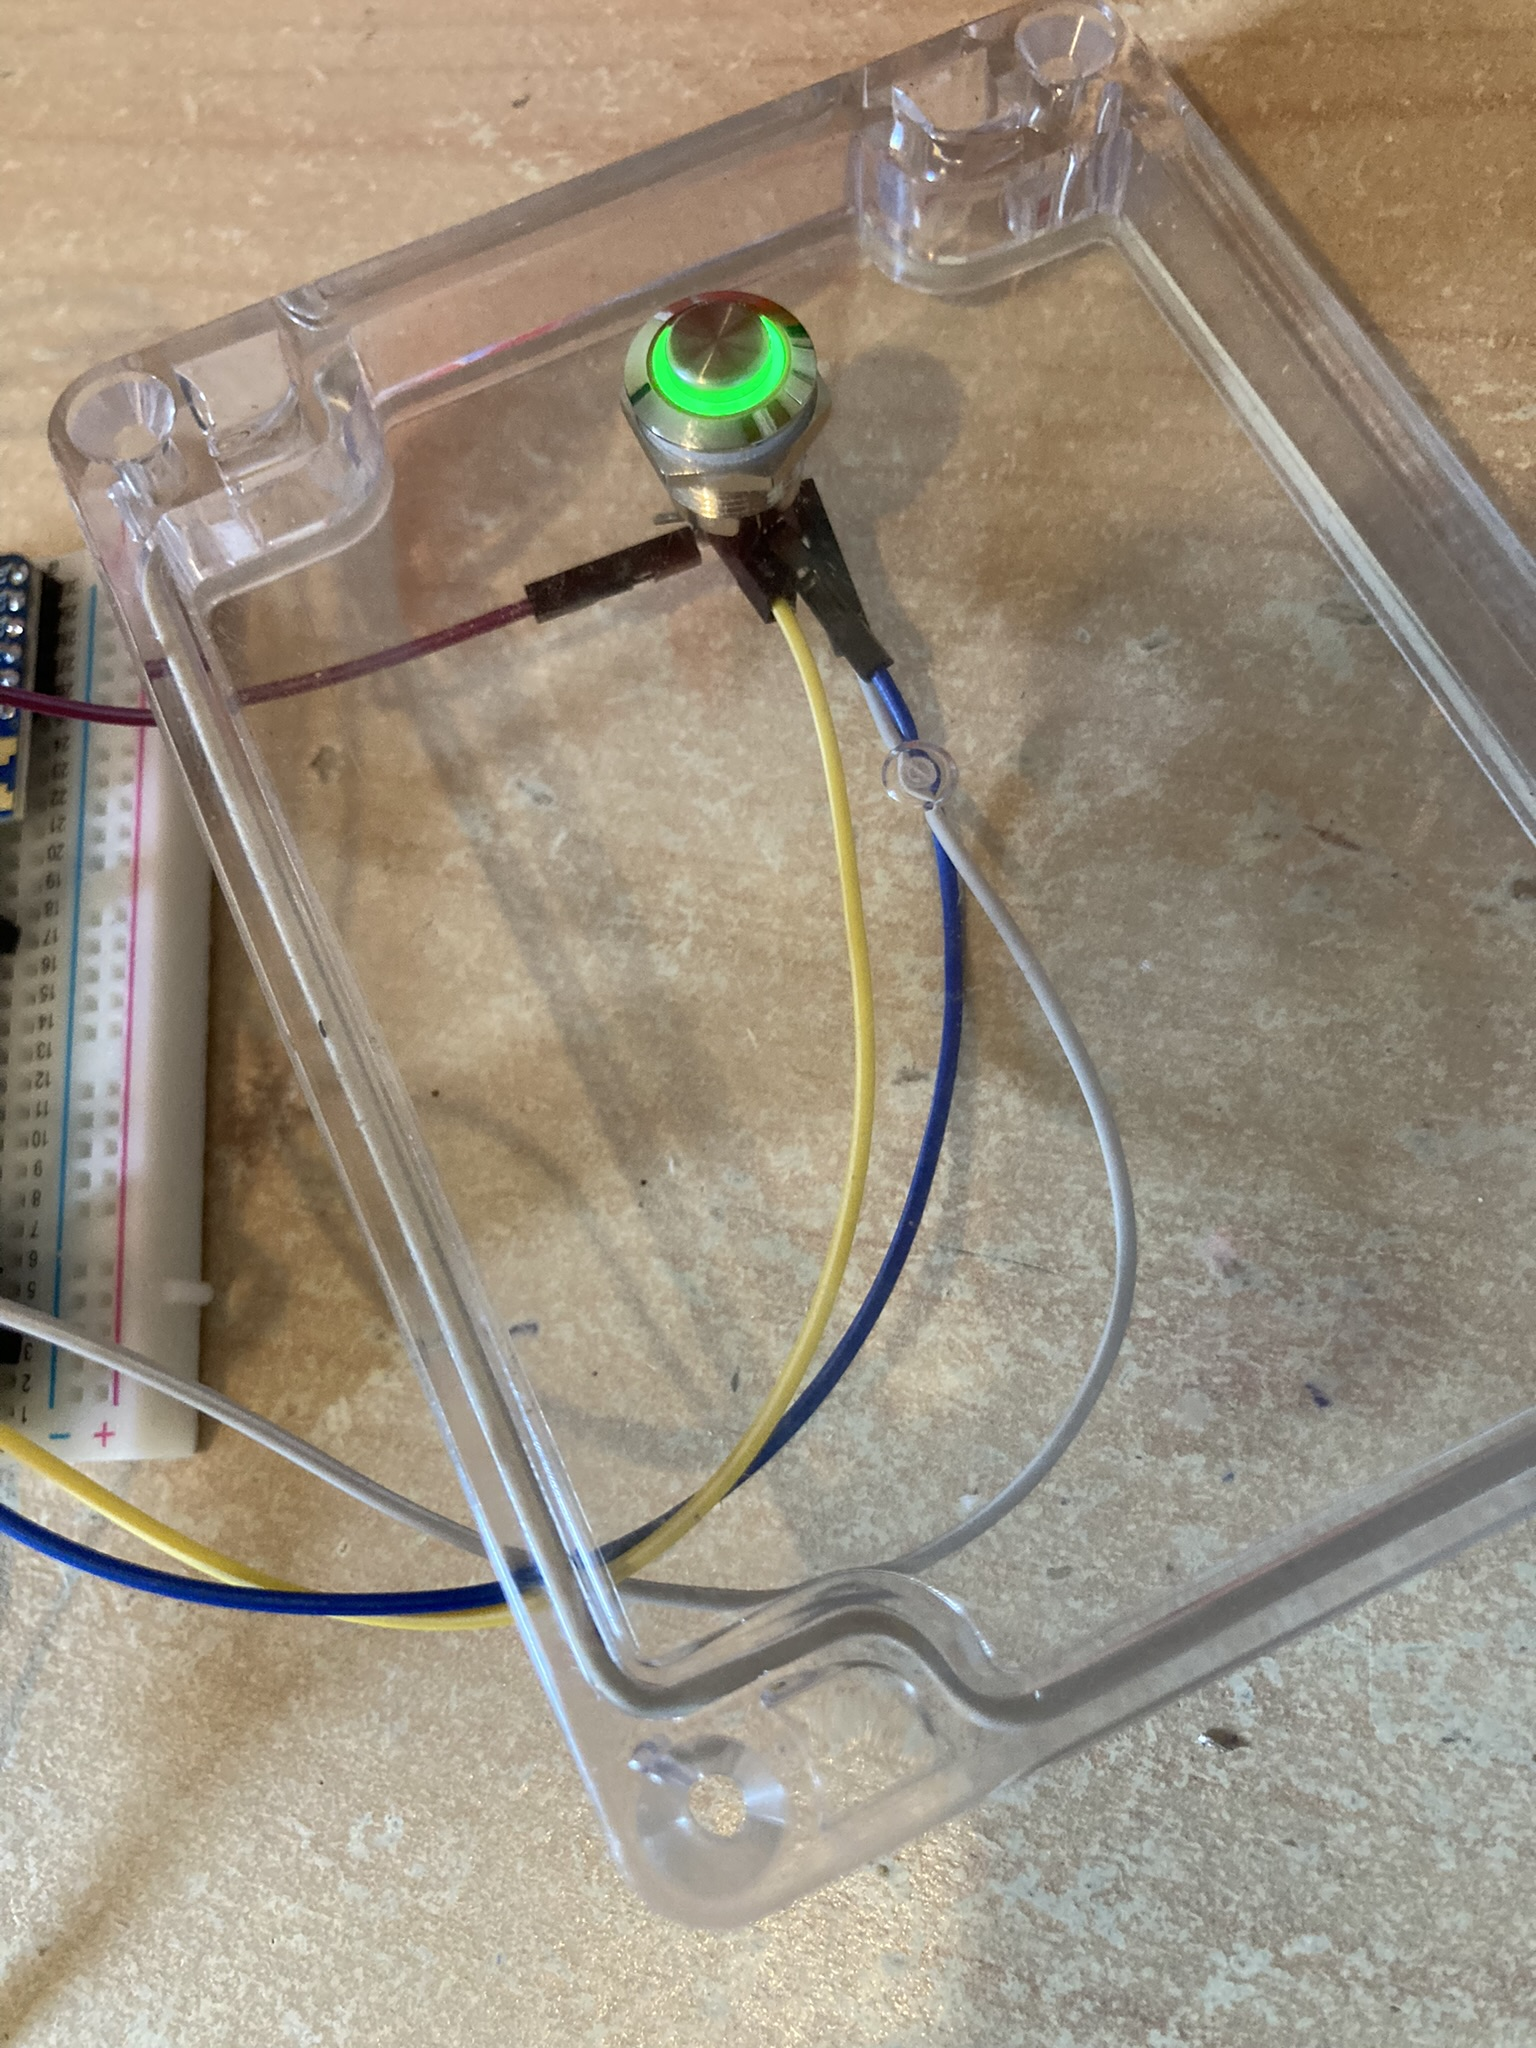
\includegraphics[scale = 0.1]{button.jpeg}
\end{center}

You'll now need to place the device into its waterproof box with a powerpack. I held all the components in place with dual lock to make sure they didn't move when inside the box. 
\begin{center}
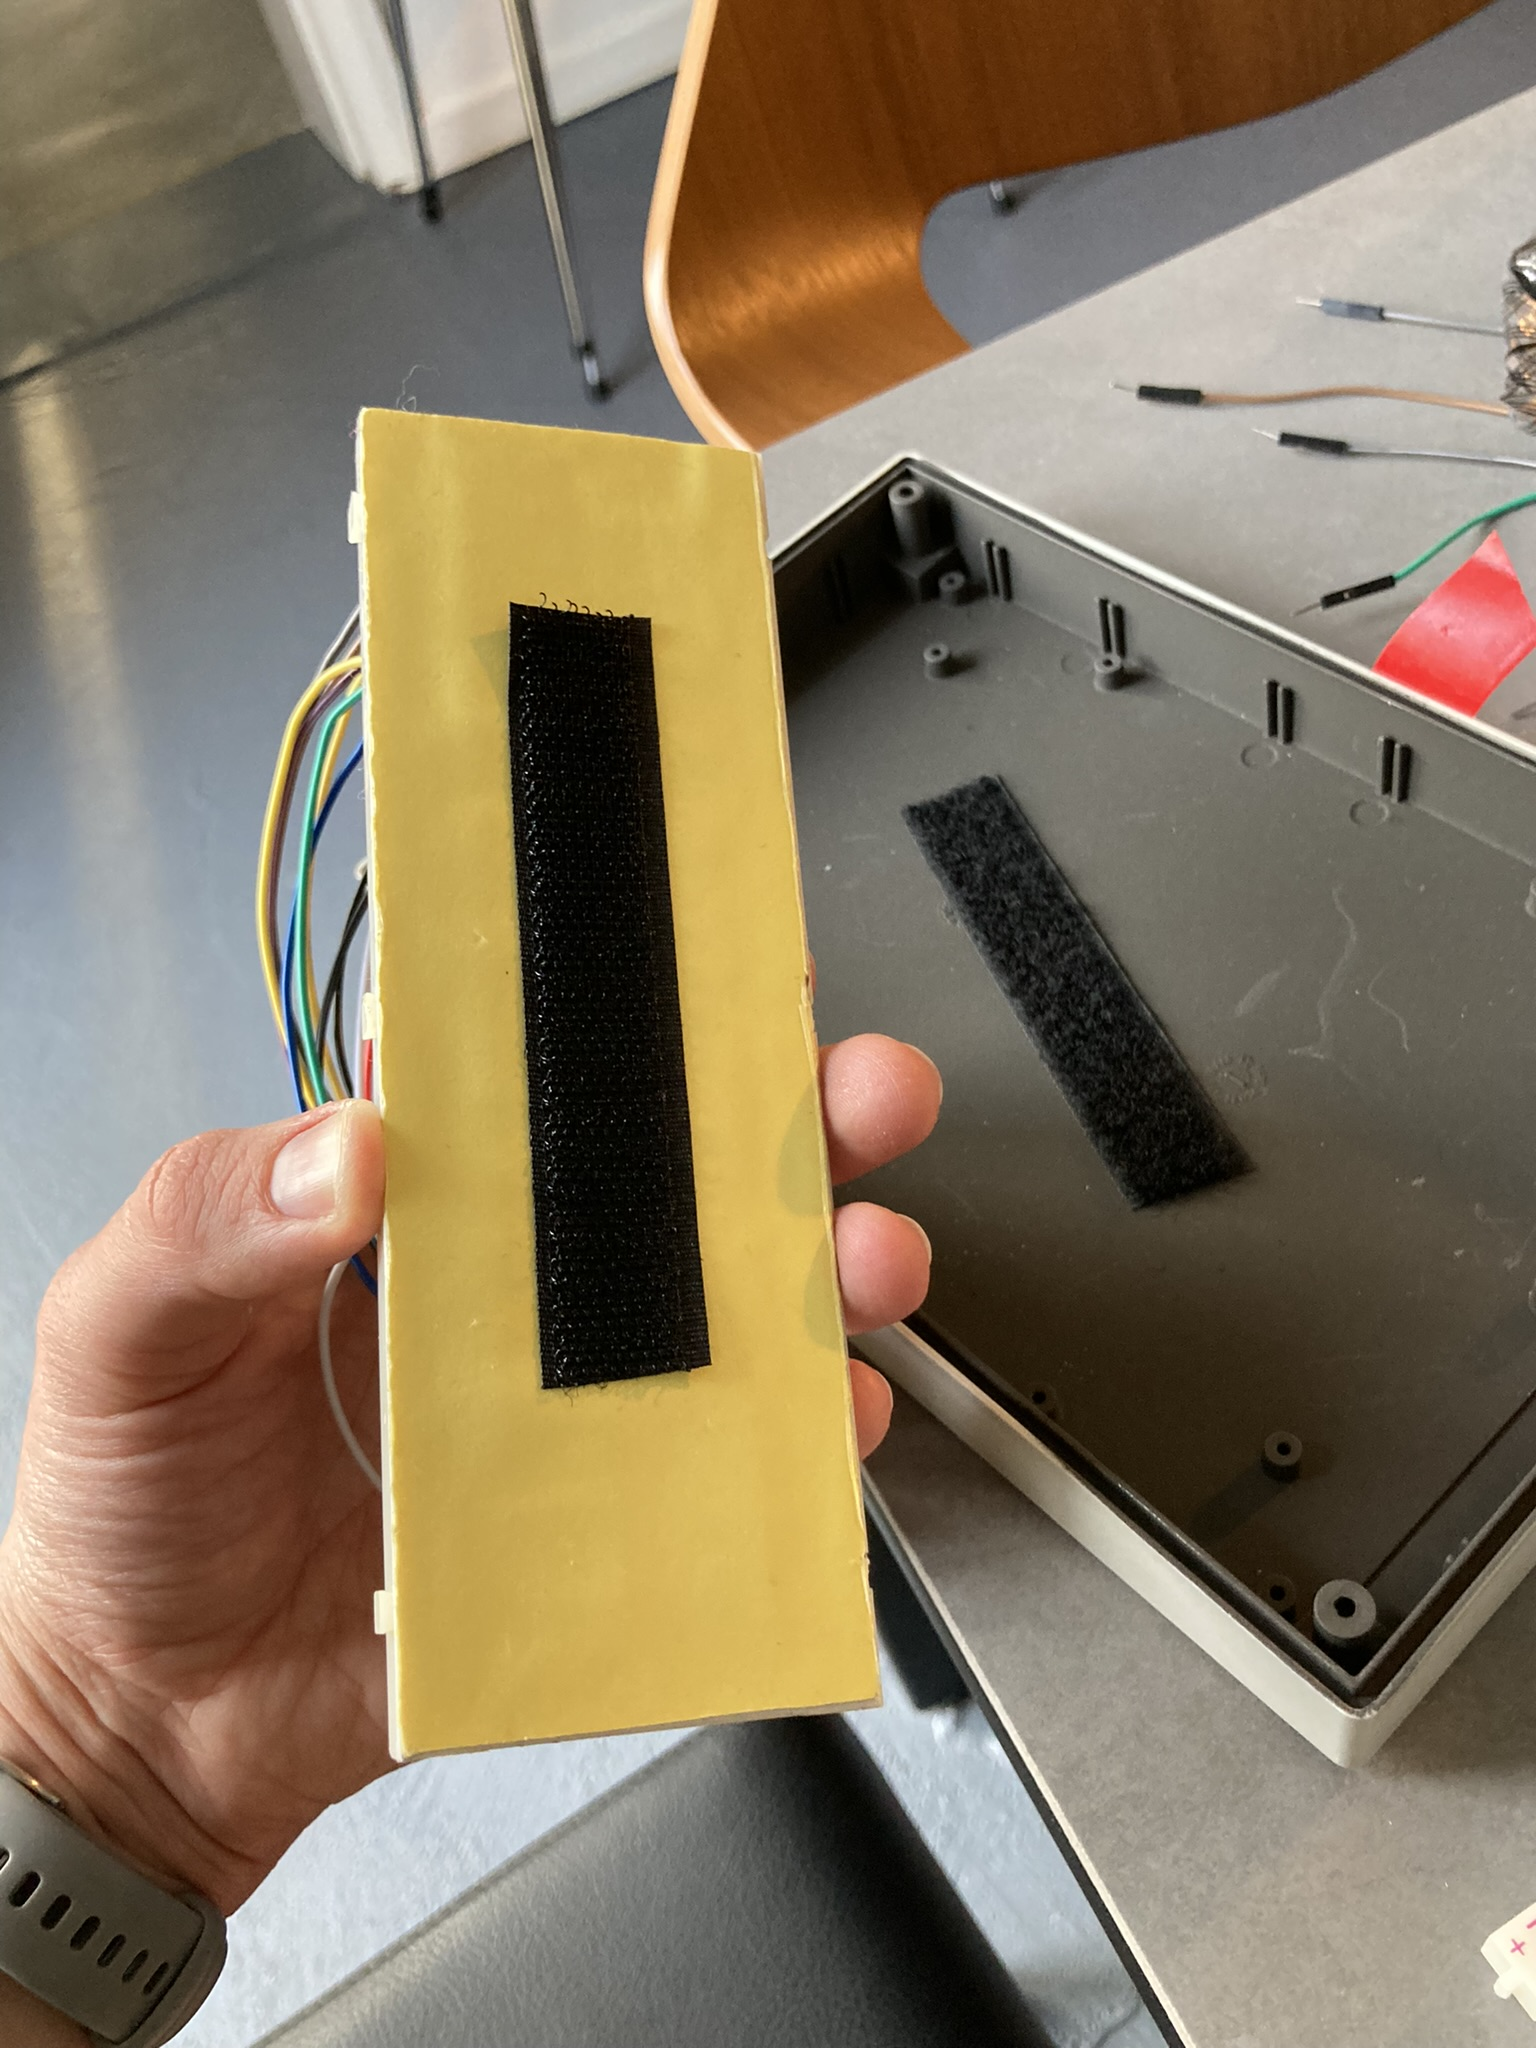
\includegraphics[scale = 0.1]{sticky.jpeg}         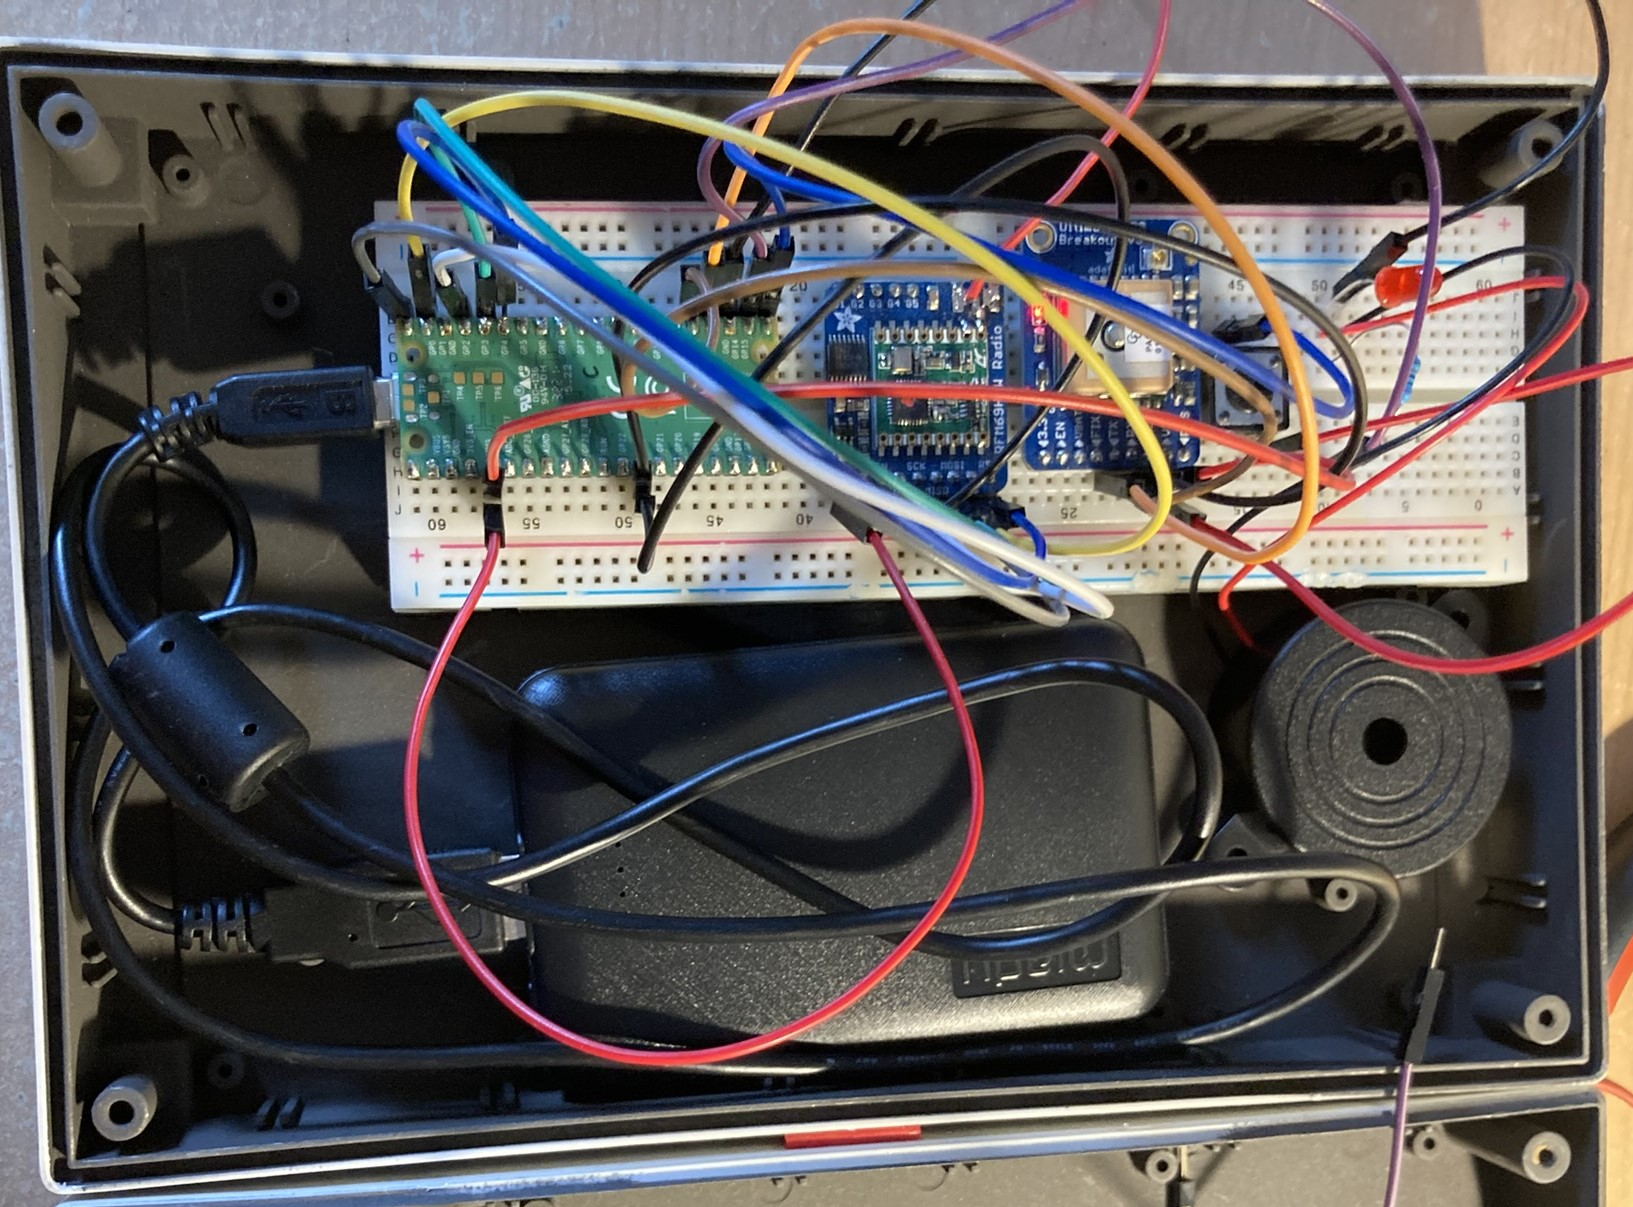
\includegraphics[scale = 0.1, angle = 90]{insideBox.jpeg} \\ \bigskip
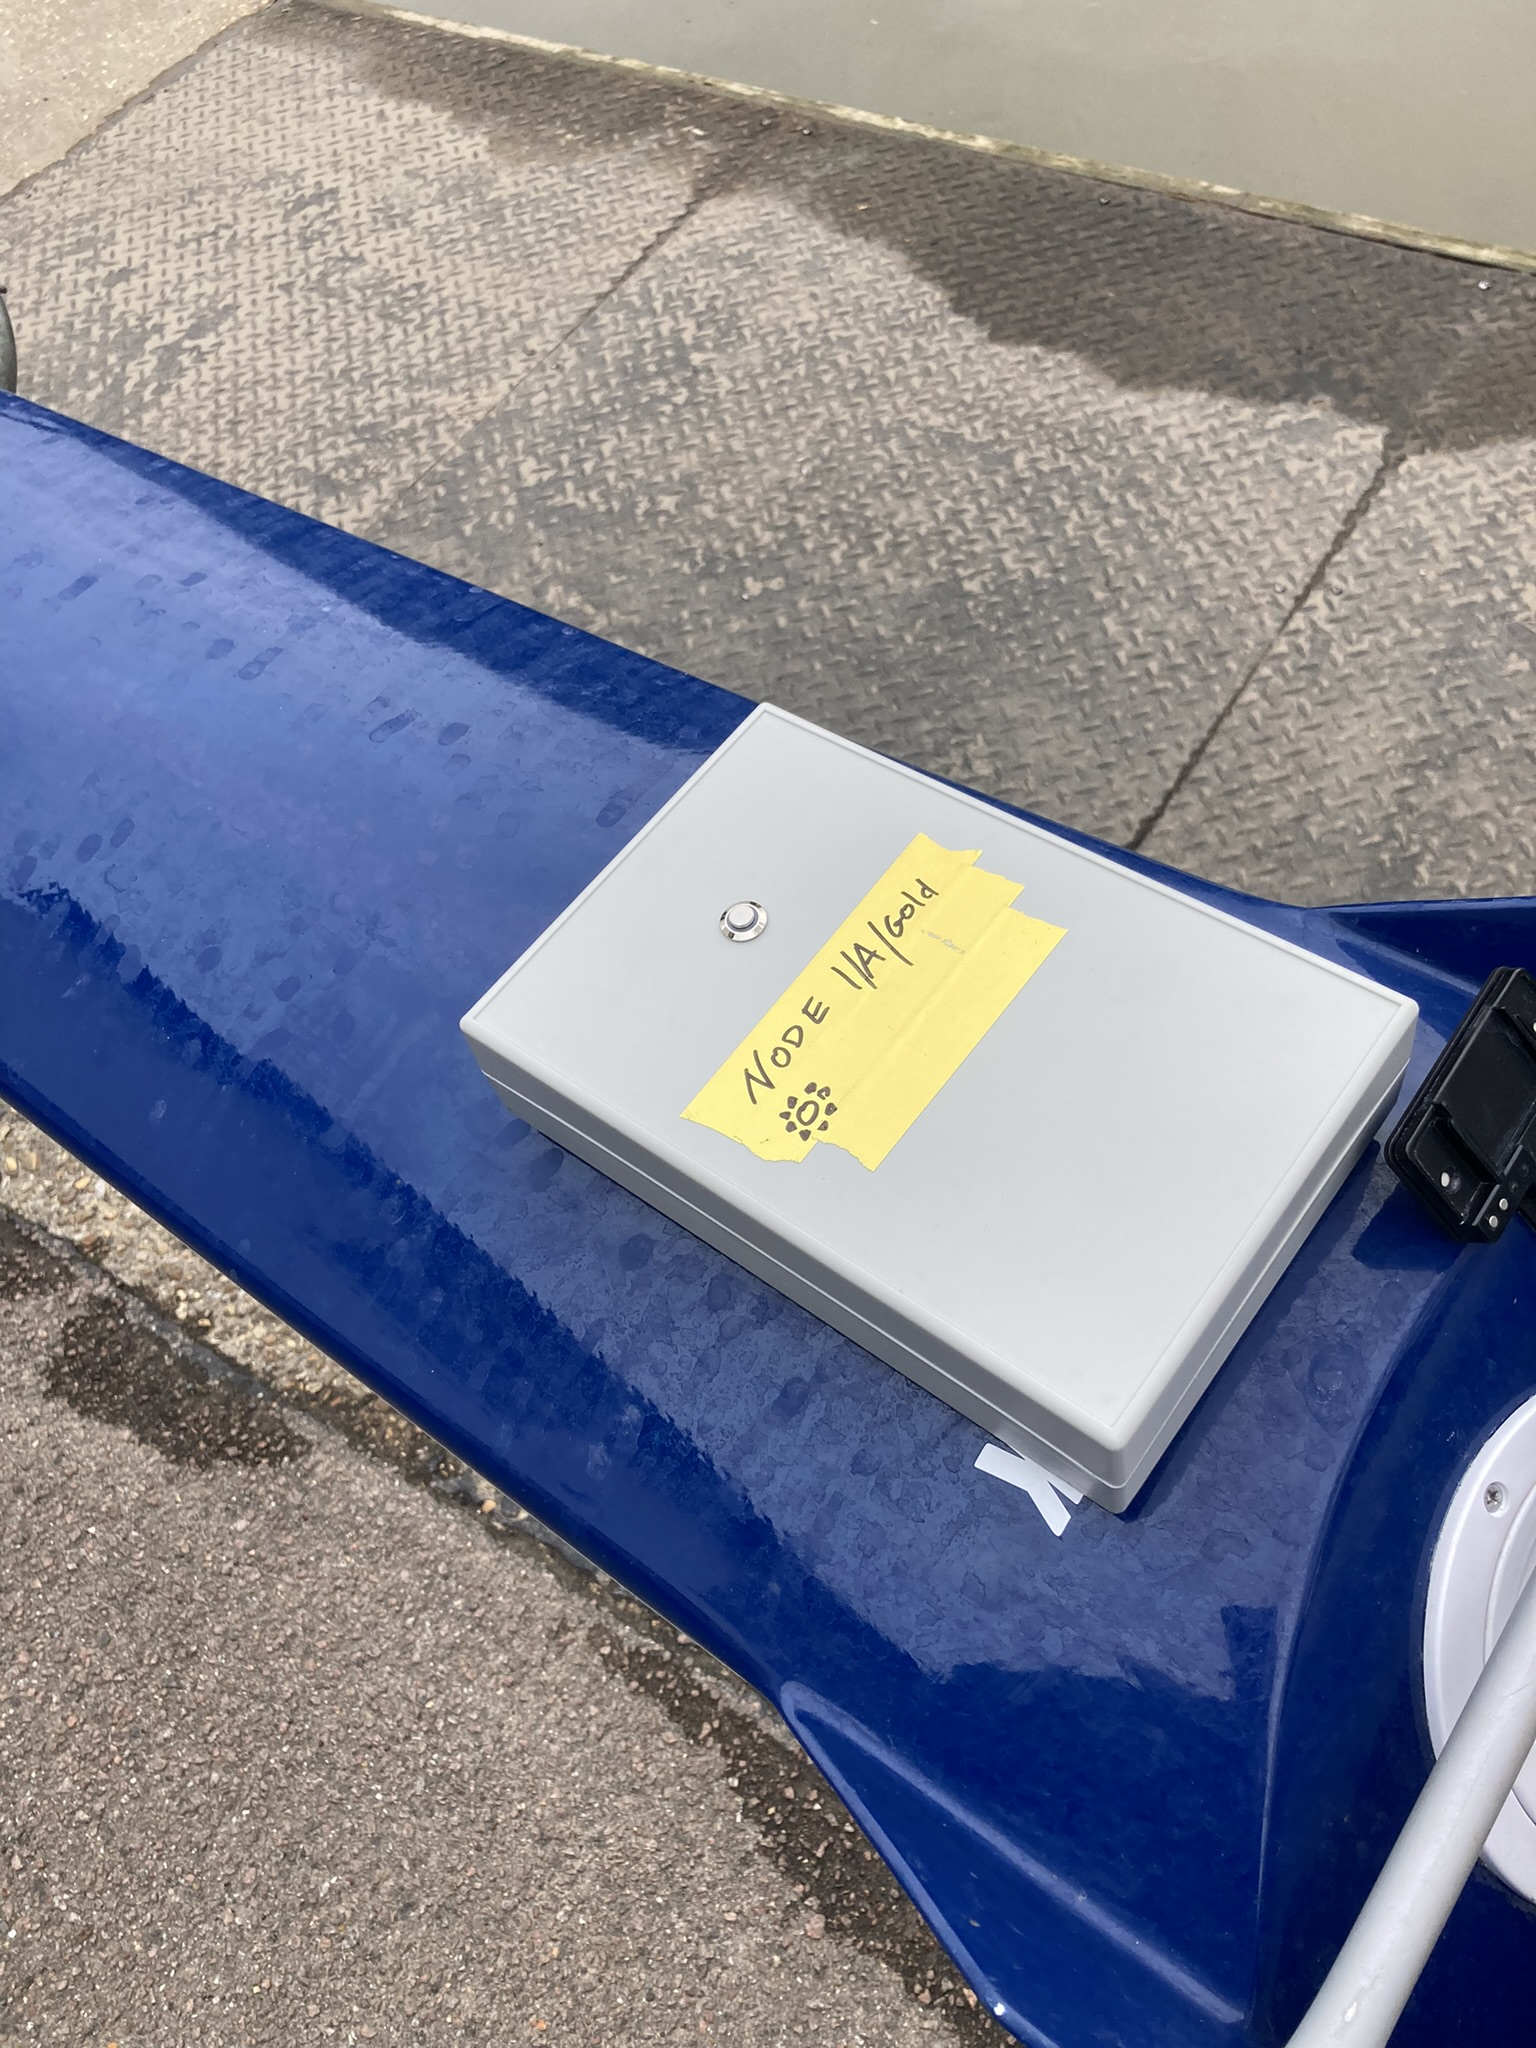
\includegraphics[scale = 0.1]{boxOnBoat.jpeg}
\end{center}

\textbf{Avoid accidents!} \\
The device should work immediately on powerup. Row safely!
\end{document}